\section{Grasping Model Architectures}

Two grasp networks were implemented and trained under the same data pipeline and loss function:
\begin{itemize}
    \item \textbf{ResNet-UNet} model
    \item \textbf{Swin Transformer} model with a lightweight multi-scale fusion decoder
\end{itemize}
Both models output three full-resolution maps: a grasp-quality logit map ($Q$ logits), and two angle maps ($\cos 2\theta, \sin 2\theta$).

\subsection{ResNet-UNet Grasp Network (ResNet34 Encoder + UNet Decoder)}

\subsubsection{Architecture Overview}
The proposed model utilizes a fully convolutional encoder-decoder architecture designed for dense, pixel-wise grasp detection. As illustrated in \textbf{Figure 3.20}, the network adheres to a U-Net-like structure but replaces the standard contracting path with a \textbf{ResNet-34} backbone. This hybrid design leverages the robust feature extraction capabilities of deep residual networks while maintaining spatial reconstruction precision through lateral skip connections. The network accepts a 4-channel \textbf{RGB-D} image as input and outputs pixel-wise maps corresponding to grasp quality and orientation parameters.

\begin{figure}[H]
    \centering
    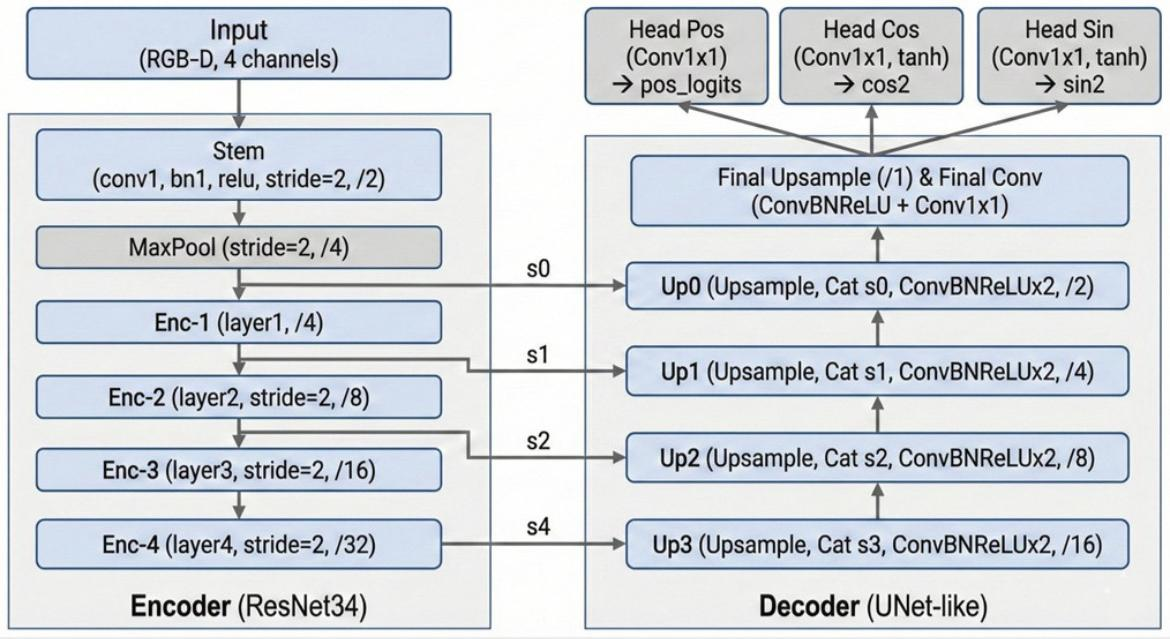
\includegraphics[width=0.8\textwidth]{Figures/chapter3/Grasping/unet_arch.jpg}
    \caption{ResNet-UNet Grasp Network (ResNet34 Encoder + UNet Decoder)}
    \label{fig:resnet_unet}
\end{figure}

\subsubsection{Feature Extraction (Encoder)}
For the encoder path, we employ a ResNet-34 model to extract hierarchical features. To accommodate the depth information crucial for geometric understanding, the first convolutional layer of the standard ResNet was modified to accept 4 input channels (RGB-D) instead of 3.

The encoder consists of an initial "stem" block (convolution, batch normalization, and ReLU with stride 2), followed by a max pooling layer and four subsequent residual stages. These stages progressively downsample the input spatial resolution by a factor of 32. This allows the network to capture high-level abstract semantic features essential for recognizing graspable objects.

\subsubsection{Upsampling and Feature Fusion (Decoder)}
The decoder path aims to recover the spatial resolution lost during encoding. It is composed of four upsampling blocks. Each block performs:
\begin{itemize}
    \item \textbf{Upsampling}: Bilinear interpolation is used to increase the feature map size by a factor of two at each step.
    \item \textbf{Feature Fusion via Skip Connections}: Upsampled features are concatenated with high-resolution feature maps from the encoder. These skip connections fuse low-level spatial details with high-level semantic features, improving the reconstruction of fine object boundaries.
\end{itemize}
Following concatenation, standard convolution layers and nonlinear activations are applied to refine the fused features.

\subsubsection{Output Representations}
The final layer branches into three distinct $1 \times 1$ convolutional heads:
\begin{itemize}
    \item \textbf{Grasp Position Head}: A single-channel score map ($Q$) representing the probability of a successful grasp at each pixel.
    \item \textbf{Grasp Orientation Heads}: Two heads output the cosine and sine of twice the grasp angle ($\cos 2\theta$ and $\sin 2\theta$). Tanh activation is applied to bound outputs between $[-1, 1]$, effectively handling angular periodicity.
\end{itemize}

\subsubsection{Implementation-Level Architecture (from resnet\_unet.py)}

The implemented ResNet-UNet model, defined by the \texttt{ResNetUNetGraspNoWidth} class, integrates a ResNet-34 encoder from \texttt{torchvision} with a U-Net-style decoder composed of four upsampling blocks and shallow output heads. The network is fully convolutional and generates three dense output maps at the same spatial resolution as the input crop: 
\begin{enumerate}
    \item[(i)] grasp quality logits (\textit{pos\_logits}) and 
    \item[(ii)] the orientation field encoded by $\cos 2\theta$ and $\sin 2\theta$.
\end{enumerate}

A primary adaptation for this project is the support for 4-channel RGB-D input ($C=4$). When using pretrained ImageNet weights, the original ResNet first convolution (conv1) is replaced with a new Conv2d(in\_channels=4, out\_channels=64, kernel\_size=7, stride=2) layer. The weights are initialized by reusing the pretrained 3-channel filters, while the additional depth channel is initialized by copying the mean of the existing RGB filters. This approach preserves the pretrained low-level feature priors while accommodating the additional depth modality.

\paragraph{Encoder/Decoder Tensor Shapes for 160$\times$160 Input}
The decoder blocks are implemented as UpBlock modules. Each UpBlock executes:
\begin{enumerate}
    \item Bilinear upsampling by a factor of 2.
    \item Channel-wise concatenation with the corresponding encoder skip feature map.
    \item Two Conv-BN-ReLU (ConvBNReLU) layers.
\end{enumerate}
This architecture restores fine spatial details lost during downsampling, which is critical for accurate grasp-center localization on small objects such as bricks.

The final feature tensor is refined by an additional ConvBNReLU(64$\to$64) followed by a $1\times1$ convolution (\textit{final\_conv}). Three separate $1\times1$ heads predict:
\begin{itemize}
    \item \textbf{pos\_logits}: No activation is applied; a sigmoid function is utilized during post-processing.
    \item \textbf{cos2/sin2}: Passed through a \textit{tanh} activation to constrain outputs to $[-1, 1]$, stabilizing the regression and maintaining consistency with trigonometric targets.
\end{itemize}

\subsubsection{Forward Pass Sequence}
The high-level forward pass logic is as follows:
\begin{equation}
    s_0 = \text{stem}(x) \rightarrow x_1 = \text{maxpool}(s_0) \rightarrow s_1 = e_1(x_1) \rightarrow s_2 = e_2(s_1) \rightarrow s_3 = e_3(s_2) \rightarrow s_4 = e_4(s_3)
\end{equation}
\begin{equation}
    d_3 = \text{up}_3(s_4, s_3) \rightarrow d_2 = \text{up}_2(d_3, s_2) \rightarrow d_1 = \text{up}_1(d_2, s_1) \rightarrow d_0 = \text{up}_0(d_1, s_0)
\end{equation}
Final operations include upsampling to $160\times160$, applying \textit{final\_conv}, and passing the result through the output heads.

\subsection{Swin Transformer Grasp Network (Swin-T Backbone + Multi-scale Fusion)}

\subsubsection{Architecture Overview}
This architecture integrates a hierarchical Vision Transformer backbone with a lightweight multi-scale fusion decoder. As illustrated in \textbf{Figure 3.21}, we utilize the Swin Transformer (Tiny variant) as the encoder. Unlike standard Vision Transformers (ViT) that utilize global self-attention, Swin Transformer constructs hierarchical feature maps by merging image patches in deeper layers.

\begin{figure}[H]
    \centering
    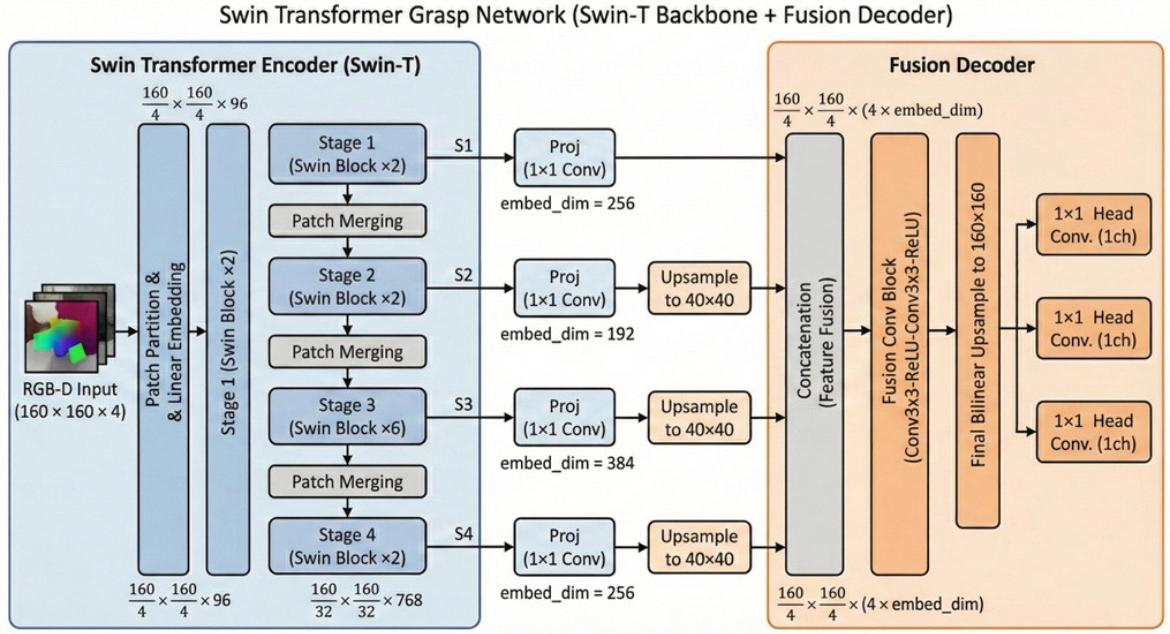
\includegraphics[width=0.9\textwidth]{Figures/chapter3/Grasping/swin_trans.jpg}
    \caption{Swin Transformer Grasp Network Architecture}
    \label{fig:swin_arch}
\end{figure}

\subsection{Swin Transformer Encoder}

The backbone follows the architectural design of Swin-T, which has a model size and computational complexity comparable to ResNet-50. The processing stages are as follows:

\subsubsection{Patch Partitioning}
The input image is split into non-overlapping patches of size $4 \times 4$. Each patch is treated as a ``token'' with a feature dimension of $4 \times 4 \times 4 = 64$ (for RGB-D input). A linear embedding layer projects this to an arbitrary dimension $C$ (where $C=96$ for Swin-T).

\subsubsection{Hierarchical Stages}
The encoder consists of four stages. To produce a hierarchical representation, ``Patch Merging'' layers are used between stages to reduce the number of tokens.

\begin{itemize}
    \item The first patch merging layer concatenates features of $2 \times 2$ neighboring patches and applies a linear layer, reducing the resolution by a factor of 2 (downsampling).
    \item This process repeats, producing feature maps at strides of 4, 8, 16, and 32 with channel dimensions of $C$, $2C$, $4C$, and $8C$ respectively.
\end{itemize}

\subsection{Window-Based and Shifted Window Self-Attention}

A key innovation of the Swin Transformer—and the primary reason for its efficiency—is the replacement of global self-attention with Window-Based Self-Attention.

\begin{enumerate}
    \item \textbf{Window-Based Self-Attention (W-MSA):} 
    Standard global attention has quadratic computational complexity with respect to the number of tokens ($O(n^2)$), which is computationally prohibitive for high-resolution images. To solve this, Swin Transformer partitions the image into non-overlapping local windows of size $M \times M$ (typically $M=7$). Self-attention is computed only within each local window. This reduces the complexity to be linear with respect to the image size ($O(HW)$), making the model much more efficient.

    \item \textbf{The Shifted Window Mechanism (SW-MSA):} 
    While W-MSA is efficient, it lacks connections across windows; tokens in one window cannot attend to tokens in a neighboring window, which limits the modeling power. To resolve this, the Shifted Window partitioning approach is employed in consecutive blocks:
    \begin{itemize}
        \item \textbf{Layer $l$ (Regular Partitioning):} The image is partitioned into regular windows starting from the top-left pixel.
        \item \textbf{Layer $l+1$ (Shifted Partitioning):} The windowing configuration is shifted by displacing the windows by $(\lfloor \frac{M}{2} \rfloor, \lfloor \frac{M}{2} \rfloor)$ pixels.
    \end{itemize}
\end{enumerate}

\paragraph{Significance}
This shift ensures that the new windows in Layer $l+1$ cross the boundaries of the windows in Layer $l$, effectively providing connections among neighboring non-overlapping windows. Consequently, the model gains the global modeling capability of standard Transformers while maintaining the linear efficiency of local windows. To compute this efficiently without padding (which would increase computation), a ``cyclic shift'' mechanism is used, where top-left blocks move to the bottom-right, allowing batched computation.

\subsubsection{Multi-Scale Fusion Decoder}
To recover spatial resolution for pixel-wise grasp detection, we implement a lightweight fusion decoder:
\begin{itemize}
    \item \textbf{Projection}: Feature maps from all four encoder stages ($S_1, S_2, S_3, S_4$) are projected via $1 \times 1$ convolutions to a unified 256-channel embedding.
    \item \textbf{Upsampling and Concatenation}: Maps are bilinearly upsampled to match the $H/4$ resolution and concatenated.
    \item \textbf{Grasp Prediction}: The fused tensor passes through a refinement block and a final upsampling to the original $160 \times 160$ resolution.
\end{itemize}

\subsection{Implementation-Level Architecture}

The implemented Swin-based model, defined in the class \texttt{SwinGraspNoWidth}, utilizes a Swin Transformer backbone integrated via the \texttt{timm} library with \texttt{features\_only=True}. The backbone exposes a pyramid of multi-scale feature maps, which a lightweight CNN fusion decoder then projects, aligns, and fuses to predict dense grasp maps at the input resolution.

\subsubsection{Input-Size Handling}
Since many Swin variants are pre-configured for $224 \times 224$ inputs, and \texttt{timm} enforces these constraints at the patch embedding layer, the backbone is explicitly initialized with \texttt{img\_size=160}. This ensures that all internal stages and the hierarchical representation are consistent with the $160 \times 160$ crops used in this project.

\subsubsection{Swin Feature Pyramid and Fusion Decoder}
In the implementation, each backbone feature map $f_i$ is processed as follows:
\begin{itemize}
    \item \textbf{Projection:} A $1 \times 1$ convolution (\texttt{ModuleList self.proj}) projects each map to a common embedding dimension.
    \item \textbf{Alignment:} All projected maps are bilinearly upsampled to the spatial resolution of the highest-resolution level, defined as $target\_hw = p[0].shape[-2:]$.
    \item \textbf{Fusion:} The aligned maps are concatenated and passed through a fusion network (\texttt{self.fuse}) consisting of two $3 \times 3$ convolutions with ReLU activations.
\end{itemize}

The fused feature map is then upsampled to the final $160 \times 160$ input resolution. Three $1 \times 1$ heads output the grasp parameters: $pos\_logits$, $cos2$, and $sin2$. While these outputs are not explicitly bounded by a $tanh$ function in this implementation, bounded behavior is maintained via target ranges and normalization within the negative-angle constraint of the loss function.

\subsubsection{Robustness to Feature Layout}
To handle variations in the \texttt{timm} library, the forward pass includes a layout check. If intermediate features are returned in $NHWC$ (Channels-Last) format, they are permuted to $NCHW$ (Channels-First) before the \texttt{Conv2d} projection to prevent channel mismatch errors.

\subsubsection{Training and Optimization}
The model is trained using the \texttt{AdamW} optimizer, which provides adaptive updates with decoupled weight decay. The primary training configurations are summarized in Table \ref{tab:hyperparameters}.

\begin{table}[h]
\centering
\caption{Training Hyperparameters}
\label{tab:hyperparameters}
\begin{tabular}{ll}
\hline
\textbf{Hyperparameter} & \textbf{Value} \\ \hline
Optimizer               & AdamW          \\
Learning Rate ($lr$)    & $1 \times 10^{-4}$ \\
Weight Decay            & $1 \times 10^{-4}$ \\
Batch Size              & 8              \\
Max Epochs              & 150            \\
Early Stopping Patience & 15 Epochs      \\ \hline
\end{tabular}
\end{table}

\paragraph{Backbone Freezing}
An optional freezing strategy is implemented. When utilizing pretrained backbones, the parameters can be frozen for the initial phase (\texttt{freeze\_epochs=5}) to allow the decoder and heads to adapt. For training from scratch, this freezing mechanism is disabled to allow for end-to-end optimization from the first epoch.

\subsection{Dataset Preparation and Label Format}
The training set consists of RGB and depth crops, each containing a single brick. Crops are generated by enlarging the detection bounding box by a fixed factor (e.g., 1.3×) to match the distribution used during dataset creation, then resizing to 160×160. For each crop, two label files are provided:
\begin{itemize}
    \item \textbf{Positive Grasps} (\texttt{cpos.txt}): Feasible grasp rectangles.
    \item \textbf{Negative Grasps} (\texttt{cneg.txt}): Invalid grasps (slipping, collision, or unstable contact).
\end{itemize}
Each label file follows a center-based format, with each line representing a single grasp rectangle as follows:
\begin{equation}
    [c_x, \quad c_y, \quad \theta_{deg}, \quad w, \quad h]
\end{equation}

Where the parameters are defined as:
\begin{itemize}
    \item $(c_x, c_y)$: The pixel coordinates of the rectangle center in the cropped image.
    \item $\theta_{deg}$: The in-plane orientation of the rectangle in degrees.
    \item $(w, h)$: The width and height dimensions of the rectangle. 
\end{itemize}



While the dimensions $(w, h)$ are stored to maintain compatibility with standard grasp-rectangle tooling, the proposed models are designed to ignore width during training, focusing exclusively on predicting grasp quality and orientation.

\subsubsection{Positive and Negative Label Handling}
Unlike conventional pipelines that remove negative samples overlapping with positive ones, this implementation retains both positive and negative rectangles regardless of spatial overlap. This approach enforces correctness through a specialized loss function that:
\begin{enumerate}
    \item \textbf{Quality Promotion:} Encourages high quality scores for locations within positive rectangles.
    \item \textbf{Quality and Angle Suppression:} Suppresses quality scores and penalizes nearby angles for locations within negative rectangles.
\end{enumerate}

This methodology allows the model to learn fine-grained orientation constraints, recognizing that specific orientations at a given location may be invalid even if other, nearby orientations are valid for a successful grasp.
\subsection{Training Objective (Loss Function)}
The total loss $L$ is defined as the sum of four terms:
$$L = L_{posQ} + L_{posAng} + \lambda_q \cdot L_{negQ} + \lambda_a \cdot L_{negAng}$$
Where:
\begin{itemize}
    \item $L_{posQ}$ is the Binary Cross Entropy (BCE) for positive grasp quality.
    \item $L_{posAng}$ is the Smooth L1 loss for angle regression on positive pixels.
    \item $L_{negQ}$ is the BCE penalty for negative-only regions.
    \item $L_{negAng}$ discourages predicted angles from approaching negative angles within a specified margin.
\end{itemize}

\subsection{Training Procedure and Implementation Details}
Both architectures are trained using the \textbf{AdamW} optimizer.

\begin{table}[H]
\centering
\caption{Training configuration used in the comparison experiments.}
\label{tab:train_config}
\begin{tabular}{lcc}
\toprule
\textbf{Parameter} & \textbf{ResNet-UNet} & \textbf{Swin-T + Fusion} \\
\midrule
Input size & $160 \times 160$ (RGB+D) & $160 \times 160$ (RGB+D) \\
Input channels & 4 (3 RGB + 1 depth) & 4 (3 RGB + 1 depth) \\
Optimizer & AdamW & AdamW \\
Learning rate & $1e-4$ & $1e-4$ \\
Batch size & 8 & 8 \\
Max epochs & 150 & 150 \\
\bottomrule
\end{tabular}
\end{table}

\subsection{ROS 2 Integration}
In deployment, the pipeline reproduces the training crop logic:
\begin{enumerate}
    \item \textbf{Detector}: YOLOv8-Seg publishes per-brick bounding boxes.
    \item \textbf{Preprocess}: Expands bbox by $1.3\times$, crops RGB-D, and resizes to $160 \times 160$.
    \item \textbf{Inference}: Runs the network and outputs the best $(cx, cy, \theta)$ grasp.
    \item \textbf{Projection}: Maps coordinates back to the 3D world frame using camera intrinsics for motion planning.
\end{enumerate}